In the rapidly evolving landscape of India's social and romantic interactions, the surge in online dating platforms like Bumble has marked a significant shift in how relationships are formed and nurtured. This shift, driven by technological advancements and changing cultural attitudes, underscores the critical importance of studying anti-discrimination within these digital realms. As internet usage in India reached an unprecedented 1.3 billion by 2023 \cite{statista_internet_users_2050}, the role of algorithms in shaping social dynamics becomes increasingly pertinent. Our research delves into the complexities of algorithmic bias and discrimination on Bumble, an online dating platform that has gained popularity among Indian users. By integrating insights from AI fairness and inclusion studies, we aim to dissect the algorithmic underpinnings that could perpetuate discrimination in the digital dating scene.

Online dating applications, which involve creating user profiles to search for and communicate with potential partners, have become a cornerstone of modern romantic and social interactions. These platforms employ various technologies, including location-based services and sophisticated algorithms, to suggest compatible partners to users. Specifically, Bumble's recommendation algorithm, which is speculated to utilize an "Elo Score" similar to that of Tinder, plays a pivotal role in this process. This score, a measure of desirability rather than mere attractiveness, is determined by a user's interaction patterns, such as "swipes" on profiles, as well as how other users interact with their profile. Despite the opacity surrounding the exact mechanics of these recommendation engines, it is evident that their effectiveness hinges on the representativeness and quality of the training data used.

However, the deployment of such algorithms raises concerns regarding the potential reinforcement of mainstream content while sidelining diverse and minority perspectives.\cite{davidson-etal-2019-racial} This issue, likely stemming from inadequate representation within the data, leads to a skewed presentation of profiles that disproportionately reflects prevailing societal preferences. The consequent narrowing of content diversity not only reinforces pre-existing cultural biases but also limits the exposure range to a homogeneous set of ideas and individuals. Our investigation into Bumble's algorithm seeks to critically evaluate how these dynamics affect interpersonal interactions and self-presentation on the platform.

Furthermore, our study places a particular emphasis on examining the discrepancies and biases in the recommendations made to individuals of dominant genders, such as men and women, compared to those identifying with non-binary genders. This exploration is crucial for uncovering any inherent algorithmic biases and discussing their broader implications for digital social interactions and inclusivity. By doing so, we aim to illuminate the ways in which digital technologies, through their algorithmic decisions, wield power and influence over social life. As this research progresses, it leads us to ponder deeper questions regarding the intersection of technology, society, and the fabric of our interpersonal relationships. Through this comprehensive analysis, we contribute to the ongoing dialogue on AI fairness and strive to foster a more inclusive digital environment where technology serves as a bridge rather than a barrier to social connectivity and understanding.

%----------------------------------------------
\section{Evolution of Dating and Matrimony Technologies}

\subsection{The West}
The history of dating and matrimony in Western societies has evolved significantly over the centuries, shaped by social, economic, religious, and technological changes. This evolution reflects broader shifts in attitudes toward marriage, gender roles, and social interactions. Pre-19th Century, marriages were arranged for political or economic alliances, and love was not considered as a prerequisite for marriage.  It was in the late 18th century that emotions and love started to play a role in matrimony. Newspapers played a crucial role in this evolution. Initially, matrimonial advertisements in newspapers were straightforward, focusing on the financial and social status of individuals seeking spouses. These ads were practical, aiming to match families for mutual economic benefit rather than love. However, as romantic love became more central to marriage, the nature of these advertisements began to change.

By the late 19th and early 20th centuries, personal ads in newspapers started reflecting the shift towards companionate marriage. These ads became more personal and emotional, with individuals describing their personal qualities, interests, and desires for a compatible partner rather than focusing solely on financial stability or social status. This change indicated a broader societal shift towards valuing emotional compatibility and love as the foundation of marriage.\cite{rothman_hands_1987}

\begin{figure}[t!]
\centering
    \subfigure[]{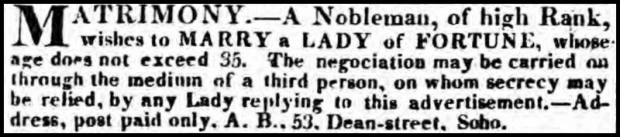
\includegraphics[width=0.45\textwidth]{figures/Introduction/morning-post-june-25-1823.png}\label{fig:img1_a}}\hfill
    \subfigure[]{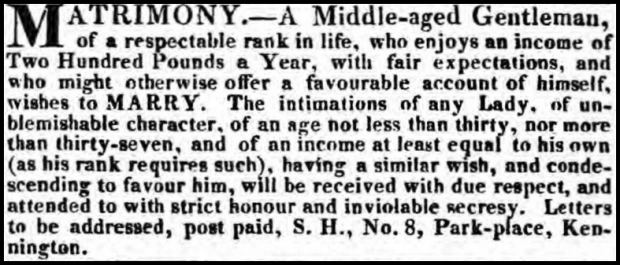
\includegraphics[width=0.45\textwidth]{figures/Introduction/morning-post-december-19-1822.png}\label{fig:img1_b}} 
    \caption{Matrimonial Advertisements in London’s \textit{Morning Post} in the 19th Century}
    \label{fig:img1}
\end{figure}

As the 19th century progressed, the popularity of matrimonial advertisements continued to grow, leading to the emergence of matrimonial specialty magazines like the Matrimonial News and the Matrimonial Intelligencer. These publications were dedicated solely to marriage and complemented the abundance of matrimonial ads found in newspapers, including those targeting specific religious audiences. Religion often played a significant role in these advertisements, highlighting the importance of shared faith in potential matches. Matrimonial ads provided an economical and accessible way for individuals who lacked family, friends, or financial resources to make meaningful connections and seek spouses.\cite{noauthor_alternative_2016}. Figure \ref{fig:img1} shows some of the examples advertisements posted in the newspapers during the 19th century. 

The concept of dating began to take shape at the turn of the 20th century, moving away from the more formal and structured courtship practices of earlier times. Dating became more informal and less focused on immediate marriage, reflecting broader social changes and evolving attitudes toward romantic relationships. This period saw the emergence of "dating" as a distinct phase of a relationship, where couples would spend time together outside the home without the immediate expectation of marriage. This shift was part of a larger cultural change that placed greater emphasis on personal choice and romantic love over social and economic considerations in mate selection. \cite{markarian_how_2017}. In the early 20th century, "Mechanical Matchmaking" emerged, with a notable example being the attempt by Hugo Gernsback, the publisher of Science and Invention magazine, to apply scientific methods to matchmaking. In April 1924, Gernsback proposed four "scientific" tests to determine the likelihood of marital success, including physical attraction tests, sympathy tests, body odor tests, and nervous disorder tests. These methods aimed to quantify and predict the success of marriages, illustrating an early fascination with applying technology and science to personal relationships, much like today's online dating algorithms.\cite{magazine_mechanical_nodate}. In the 1950s, a Newark based, matchmaking service called Introduction, used data as a foundation of their matchmaking services and charged a fee for ‘personalized’ recommendations of suitable matches based on qualifications and social status and subsequent sharing of contact information. \cite{newark_introduction_nodate}

One landmark development in the fusion of technology and dating was Operation Match, which emerged from Harvard University in 1965. Developed by undergraduate students Jeff Tarr and Vaughan Morrill, along with Doug Ginsberg and David Crump, Operation Match was conceived as an innovative solution to the challenges of dating life on campus. Utilizing an IBM 1401 computer, the service employed a sophisticated algorithm to match individuals based on their responses to a comprehensive questionnaire covering personal preferences and interests.\cite{noauthor_operation_1965}  Participants of Operation Match filled out lengthy questionnaires, which they submitted with \$3, and a program on an IBM 1401 computer would match questionnaires to similar responses.\cite{valley_new_2015}  The questionnaires were then transferred to punched cards and processed on an IBM 7090 computer and users received an IBM 1401 print out in the mail a week later, listing the names and contact information of potentially suitable matches. The increased sophistication provided by the IBM 1400 series propelled computer matchmaking into the public shhere as commercial matchmaking servics adopted advanced means to help singles find suitable dates. This increase in popularity of preferenced based match making combined with sexual revolution of the 1960s and 1970s, because of the introduction of oral contraceptives in the 1960s, the rising visibility of the LGBTQ+ community along with the second-wave of feminist movement,\cite{book:1309549} brought upon a drastic change in the attitudes of the people towards dating and relationships. From a culture that only endorsed serious relationships and marriage with the flexibility to choose a sociall equivalent partner, the society started to accept casual dating and hookups. The culture encouraged an individual to explore for their options both sexually and romantically, with multiple partners without any restrictions based on social strata and also having no end goal of marriage. The emergence of modern dating practices offered unprecedented opportunities for social mobility and the exploration of sexuality, albeit within the constraints of the era. This development represented a significant departure from traditional expectations, which often confined individuals to relationships with partners from specific, socially sanctioned groups. Women, in particular, experienced a notable expansion of autonomy through the relaxation of socio-cultural restrictions\cite{book:1309549}. This newfound freedom enabled them to date, form romantic attachments, and partake in sexual relationships with greater agency. 

\begin{figure}[t!]
 \centering
 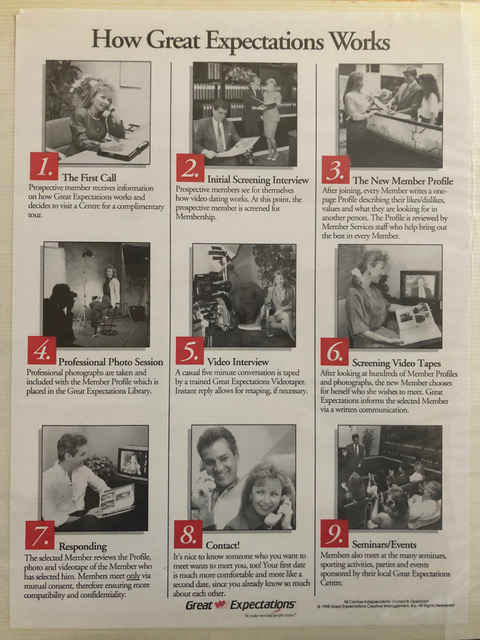
\includegraphics[scale=0.6]{figures/Introduction/GE2.png}
 \caption{A flyer explaining how Great Expectations works}
 \label{fig:img2}
\end{figure}

In the 1980s, post the rise of computer matchmaking, video matchmaking started to emerge. Video (or VHS) dating brought along with it a new way to meet potential partners, with added dimension of being able to hear and see the person before meeting them in person. The first known video dating service was started by Jeffrey Ullman in 1983, called the Great Expectations.\cite{waters_how_2021}. In video matchmaking, participants were asked a series of personal and motivational questions, such as their work ethic, triggers for anger, sources of motivation, and qualities they sought in a partner. After these interviews were recorded, the videotapes were cataloged in a video dating library. Members could browse through this collection, aided by a one-page profile attached to each video that included key details like height, location, and occupation, allowing them to screen potential matches before watching a tape. Figure \ref{fig:img2}, shows a flyer explaining how Great Expectations works. Hearing and Viewing the partners before selecting them was a significant advantage, because as Ullman said ``it showcased a more honest version of a person". \cite{waters_how_2021} This method brought out some of the marvellous personalities of people that would not show up just based on a written questionnaire as was the case in the previous approaches. But the hype of video dating dwindled in the early 1990s because of how cumbersome the process was. It did not bring out a massive change in the dating culture, but it did pave the way for the design of modern dating applications. 

The terminology "matchmaking" is purposefully employed in the preceding sections to delineate pre-Match.com "dating" mechanisms, as these early technologies primarily served the function of facilitating introductions between two parties deemed compatible on a multitude of criteria, ranging from social status to individual predilections and shared ideologies. Prior to the digital revolution instigated by Match.com, "dating" technologies were constrained to the matchmaking domain, enabling initial introductions without encompassing the subsequent phase of dating, which is crucial for assessing compatibility through real-world interactions. The advent of the internet, and specifically Match.com, heralded a paradigm shift by amalgamating matchmaking and dating within a unified online platform. Match.com was instrumental in revolutionizing the dating industry by accelerating the matchmaking process and introducing communication features like chat boxes, thereby allowing matches to engage in preliminary interactions ('date') prior to arranging face-to-face encounters.\cite{noauthor_dating_nodate} This platform introduced the concept of a 'dating profile', encouraging users to provide personal insights alongside photographs, thereby streamlining the process of discovering and interacting with potential matches within a singular service. Contrasting with prior methodologies, which necessitated intermediary involvement and were characterized by significant delays, online dating platforms provided immediate access to an expansive pool of potential matches, along with the autonomy to evaluate compatibility through direct communication, thus enhancing the process's transparency, dynamism, and efficiency.

The evolution of dating technologies further advanced with the development of mobile dating applications, such as Tinder and Bumble, transforming the dating experience into a mobile-centric endeavor. These applications, extensively discussed in the second chapter, innovated user interaction through the implementation of the 'swipe' mechanism and a pronounced focus on visual self-presentation\cite{noauthor_dating_nodate, marcus2016swipe} Notably, such applications significantly contributed to normalizing the sexual exploration or 'hook-up' culture, making it openly accessible and socially acceptable across various demographics\cite{noauthor_dating_nodate, marcus2016swipe}. Tinder, for instance, played a pivotal role in normalizing explicit expressions of sexual intentions by incorporating features that allow users to specify their looking-for preferences, such as casual encounters or long-term relationships, directly on their profiles. Employing sophisticated algorithms and engaging chat functionalities, including emojis, GIFs, and memes, these applications further refined the match screening process, enabling users to make more informed decisions regarding the viability of face-to-face meetings.

This transition from traditional matchmaking services to comprehensive online dating platforms has significantly broadened the interaction spectrum, empowering users to exercise greater selectivity in their dating pursuits. By facilitating a virtual screening process, these digital mediums have not only conserved time and effort but have also expanded the horizons for establishing and nurturing romantic connections in the contemporary era, underscoring a profound shift in the landscape of dating technologies.


\subsection{The Indian Context}
The evolution of dating and matrimony technologies in India has been influenced by the country's unique socio-cultural landscape, characterized by a rich tapestry of traditions, values, and familial structures. It is evident from the previous section that the Western dating culture has undergone significant transformations over the centuries, transitioning from arranged marriages to companionate marriages and subsequently embracing casual dating and hook-up culture. In contrast, to the technologies in the west, dating technology were modified to server as matrimonial services because of the social unacceptability of any form of Dating in the Indian society, until the 2000s \cite{doshi_date_2016, noauthor_modern_2017, sharma_towards_2019}. 

Traditionally, personal advertisements were predominantly utilized to identify appropriate marital alliances, and the inception of Shaadi.com, shortly after the launch of Match.com, mirrored this utility, albeit within the matrimonial context of Indian society. In this cultural milieu, the responsibility of selecting suitable marital candidates traditionally rested with the parents, given the substantial emphasis placed on variables such as caste, religious affiliation, and upbringing. These factors not only held, but continue to hold, considerable importance, with parents extensively relying on their expansive social networks to discover apt matches for their offspring \cite{sharma_towards_2019, seth_online_2008}. Matrimonial services remained largely unchanged, focusing predominantly on matchmaking, as the prerogative to sift through recommended matches was vested in the parents of the concerned individuals, thereby obviating the necessity for incorporating 'dating experiences' to vet multiple prospective partners \cite{titzmann_changing_2013}. The paramount decision-making authority resided with the parents, thus constraining opportunities for dating or romantic exploration—until the widespread adoption of mobile phones in the early 2000s. Mobile telephony and the internet introduced novel avenues for discreet dating, facilitating the quest for partners beyond the traditional constraints of caste and religious affiliations. It is pertinent to highlight that, at this juncture, the Indian dating paradigm mirrored Western practices of the early twentieth century, predominantly aimed at culminating in 'love marriages.'

The landscape of Indian dating culture witnessed a profound transformation in 2011 with Tinder's entry into the Indian market. Marketed primarily as a 'hook-up' application, Tinder swiftly gained traction among the youth, thereby democratizing dating and, notably, casual romantic encounters. The prevailing narratives suggest a gradual shift from a staunchly arranged marriage-oriented society towards a more open acceptance of 'dating' among the younger demographic. This cultural evolution is fostering the emergence of varied dating practices, spanning from serious relationships to casual dating and hook-ups. The locus of choosing a partner is increasingly transitioning from parents to the individuals themselves, buoyed by the rising popularity of online dating platforms such as OkCupid and Tinder. This paradigm shift towards individual agency in partner selection is a relatively recent development, with online dating gaining the quickest acceptance among college students and young professionals \cite{doshi_date_2016}.
